\documentclass[page number]{beamer}
\usetheme[sectionpage=none,numbering=fraction,progressbar=foot]{metropolis}

\usepackage{pgf,tikz}
\usetikzlibrary{arrows}
\usetikzlibrary{positioning,shapes,fit}
\usepackage{xcolor}
\usepackage{amssymb}
\usepackage{amsmath}

\makeatletter
\makeatother

\setcounter{tocdepth}{1} % remove subsection from table of contents

% colors
\definecolor{mDarkRed}{HTML}{6F1616}
\definecolor{mDarkGreen}{HTML}{106235}
\definecolor{mTeal}{HTML}{112233}
\definecolor{mBlack}{HTML}{000000}
\setbeamercolor{normal text}{fg=mTeal}
\setbeamercolor{alerted text}{fg=mDarkRed}
\setbeamercolor{example text}{fg=mDarkGreen}
\setbeamercolor{title separator}{fg=purple,bg=mBlack}

\definecolor{spec}{HTML}{6F1616}
\definecolor{prog}{HTML}{106235}

\def\outline{
  \begin{frame}[plain,noframenumbering]
    \frametitle{Outline}
    \tableofcontents[currentsection]
  \end{frame}
}


\begin{document}
\title[Pretty Big Step]{Pretty-Big-Step Semantics}

\author[Aur\`ele Barri\`ere]{Aur\`ele Barri\`ere}

\date{\textbf{December 7, 2018}}

\def\outline{
  \begin{frame}[plain,noframenumbering]
    \frametitle{Outline}
    \tableofcontents[currentsection]
  \end{frame}
}

\begin{frame}[plain,noframenumbering]
  \vspace{-2cm}
  \maketitle
  \vspace{-4cm}
\end{frame}

%% \metroset{sectionpage=none}

%% \metroset{sectionpage=progressbar}

\begin{frame}{Pretty-Big-Step Semantics}
  \begin{itemize}
  \item Operational Semantics.
  \item Inspired by Big-Step Semantics.
  \item Choosing a Semantics' style is about the way of writing the rules and doing the proofs, not expressivity.
  \end{itemize}
  \vfill
  \begin{alertblock}{Small-Step Semantics}
    Step: $(\mathit{code},\mathit{State})\rightarrow(\mathit{code},\mathit{State})$.\\
    Many steps until final configuration.
  \end{alertblock}
  \vfill
  \begin{exampleblock}{Big-Step Semantics}
    One step: $(\mathit{code},\mathit{State})\rightarrow\mathit{State}$.
  \end{exampleblock}
  
\end{frame}

\begin{frame}{Small-step Reminder}
  \center
  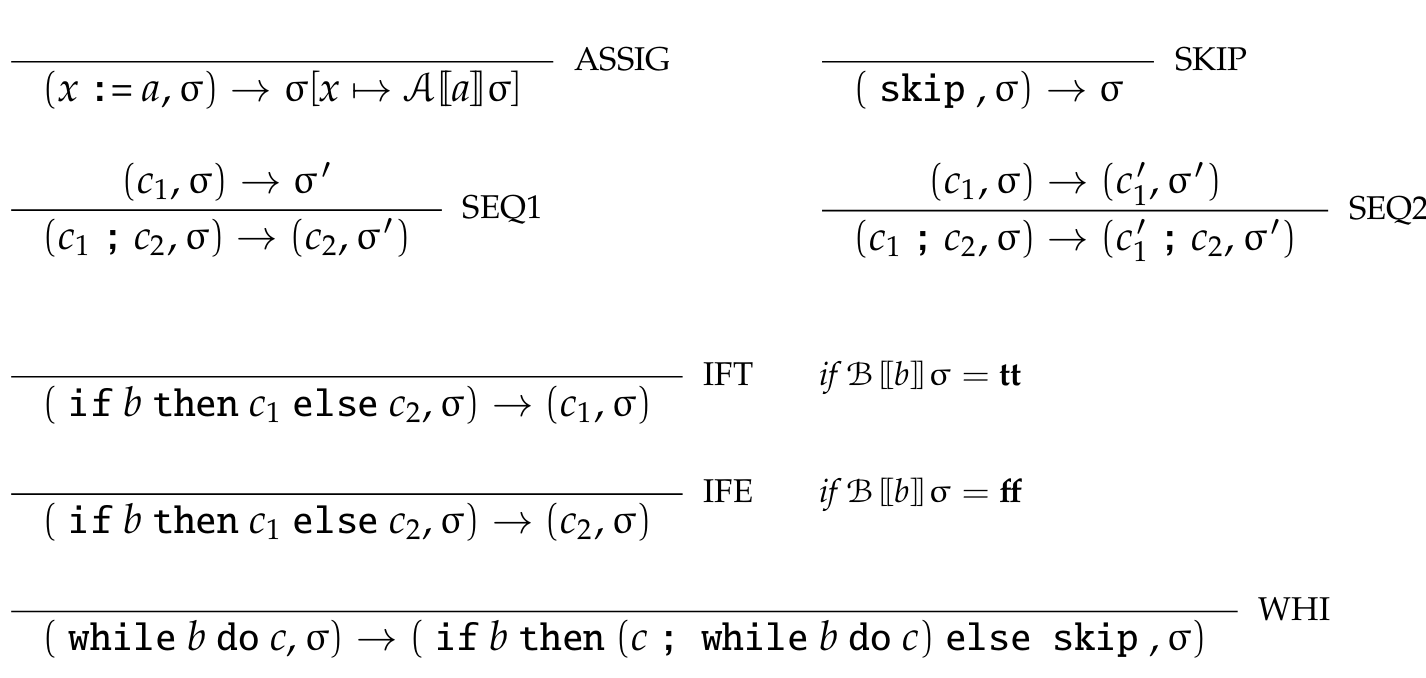
\includegraphics[scale=0.2]{smallstep.png}
\end{frame}

\begin{frame}{Big-step Reminder}
  \center
  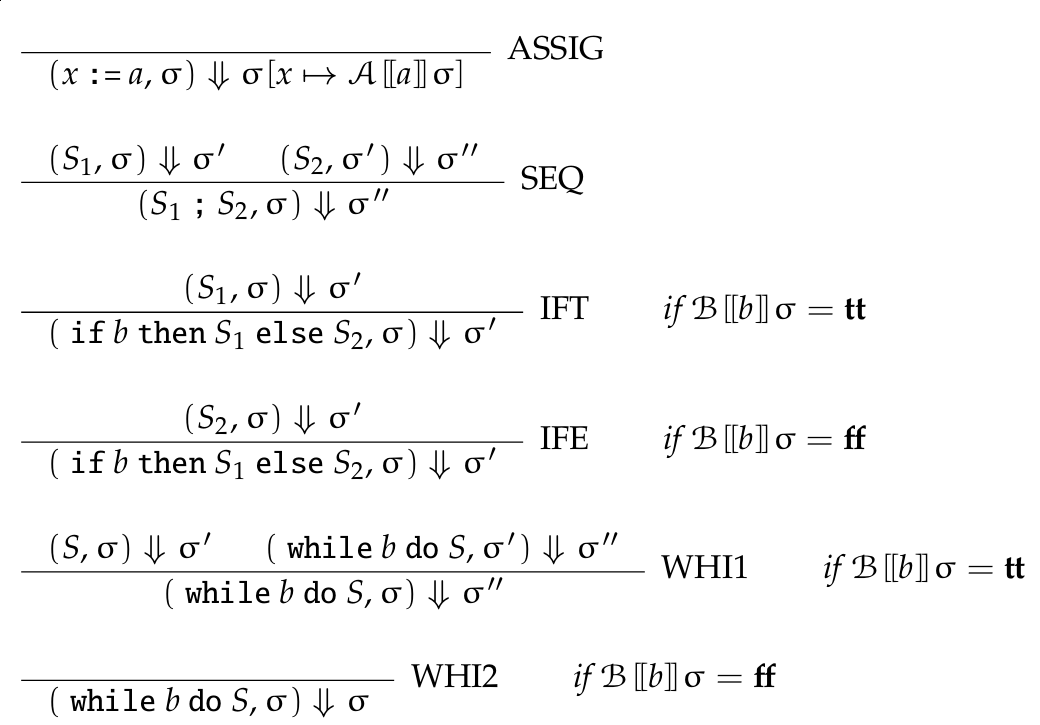
\includegraphics[scale=0.2]{bigstep.png}
\end{frame}


\begin{frame}{Why Pretty-Big-Step Semantics?}
  \begin{block}{Big-Step is still used}
    \begin{itemize}
    \item 17 out of 40 operational semantics in recent conferences.
    \item Cost semantics, informal description.
    \item Some proofs need to be done on big-step semantics.
    \end{itemize}
  \end{block}
  \vfill
  \begin{alertblock}{Drawbacks of Big-Step Semantics}
    Redundancy when adding new constructs.\\
    For instance: divergence, errors, control-flow exceptions\dots
  \end{alertblock}
\end{frame}

\begin{frame}{Duplicating rules in Big-Step Semantics}
  The example of divergent behavior.\\
  \center
  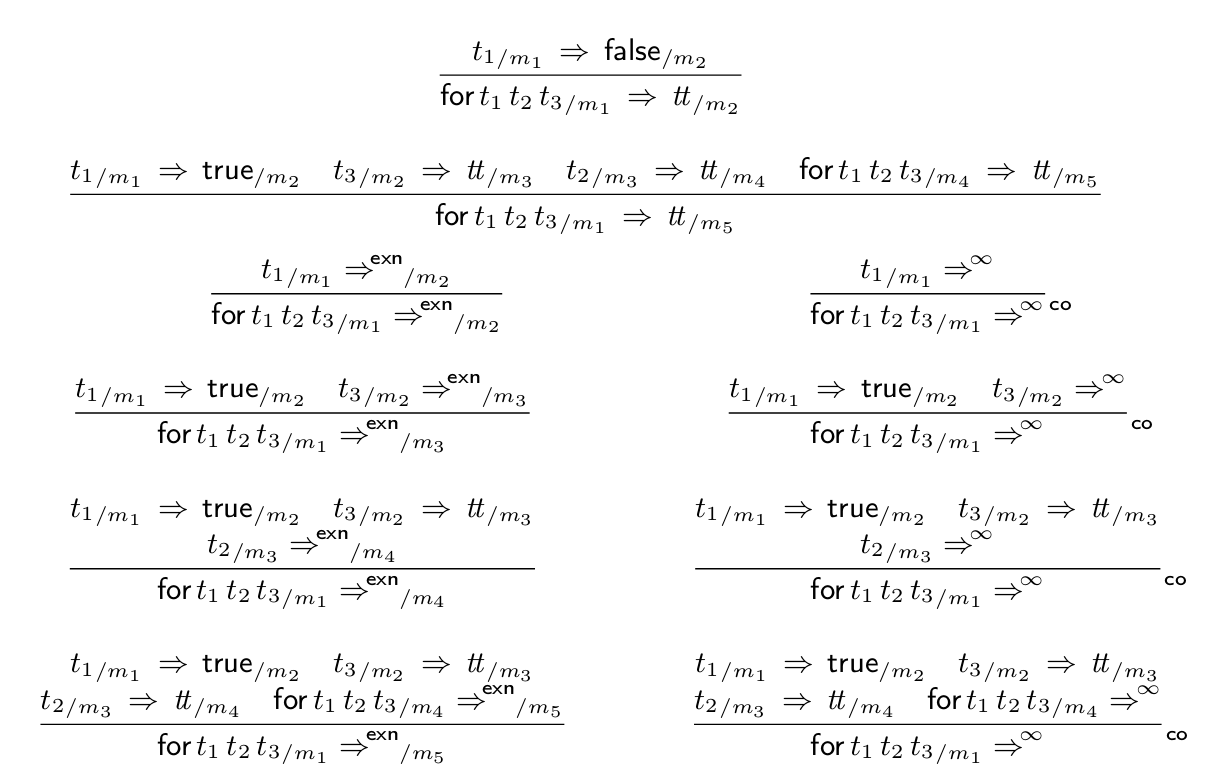
\includegraphics[scale=0.25]{duplicates.png}
  
\end{frame}

\begin{frame}{Pretty-Big Step Presentation}
  \begin{exampleblock}{Properties}
    \begin{itemize}
    \item less rules.
    \item no duplication of premises.
    \item use coinduction for diverging behaviors.
    \item add intermediate terms
    \end{itemize}
  \end{exampleblock}
  \vfill
  \begin{block}{Example: $\lambda$-calculus}
    \center
    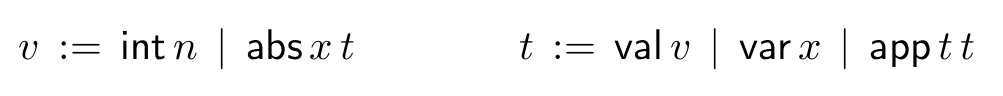
\includegraphics[scale=0.3]{lambda.png}
  \end{block}
\end{frame}

\begin{frame}{Evaluating Application}
  \begin{alertblock}{Big-Step}
    \center
    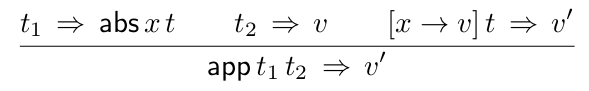
\includegraphics[scale=0.3]{bigstep_betared.png}
  \end{alertblock}
  \vfill
  \begin{block}{First Attempt at Pretty-Big-Step}
    \center
    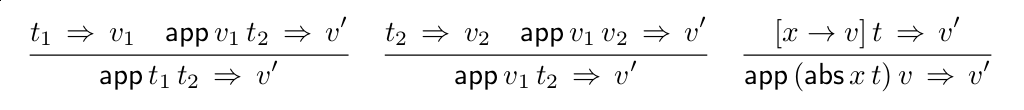
\includegraphics[scale=0.3]{first_attempt_betared.png}
  \end{block}
  \begin{alertblock}{Overlapping Problem}
    Evaluation isn't syntax-directed.
  \end{alertblock}
\end{frame}

\begin{frame}{Intermediate Terms}
  \begin{block}{Term Syntax}
    \center
    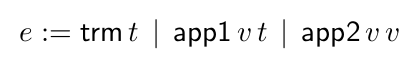
\includegraphics[scale=0.3]{interm.png}
  \end{block}
  \vfill
  \begin{exampleblock}{Non-overlapping Semantics}
    \center
    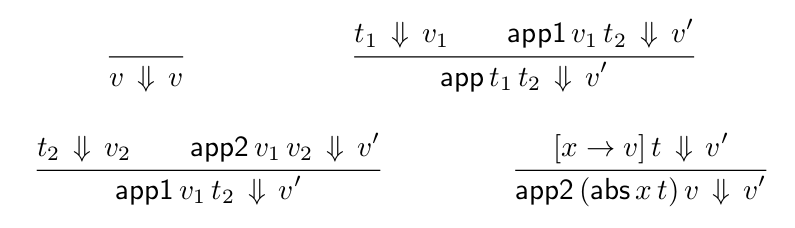
\includegraphics[scale=0.3]{interm_step.png}
  \end{exampleblock}
\end{frame}

\def\app{\mathbf{app}}
\def\abs{\mathbf{abs}}
\begin{frame}{Example}
  Evaluation of $(\lambda y.~ (y ~0))~ (\lambda x.~ x + 2)$.\\
  $\app~(\abs~ y~ (\app~ y~ 0))~(\abs~ x~ (x+2)))$.
  \vfill
\end{frame}


\begin{frame}{Exceptions}
  \begin{block}{Generalized Behavior and Extended Intermediate Terms}
    \begin{center}
    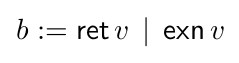
\includegraphics[scale=0.3]{behavior.png}\hfill
    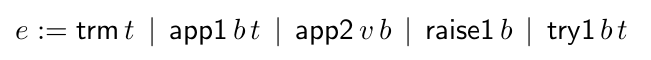
\includegraphics[scale=0.3]{expr_ex.png}
    \end{center}
  \end{block}
  \vfill
  \begin{exampleblock}{Pretty-Big-Step Rules}
    \center
    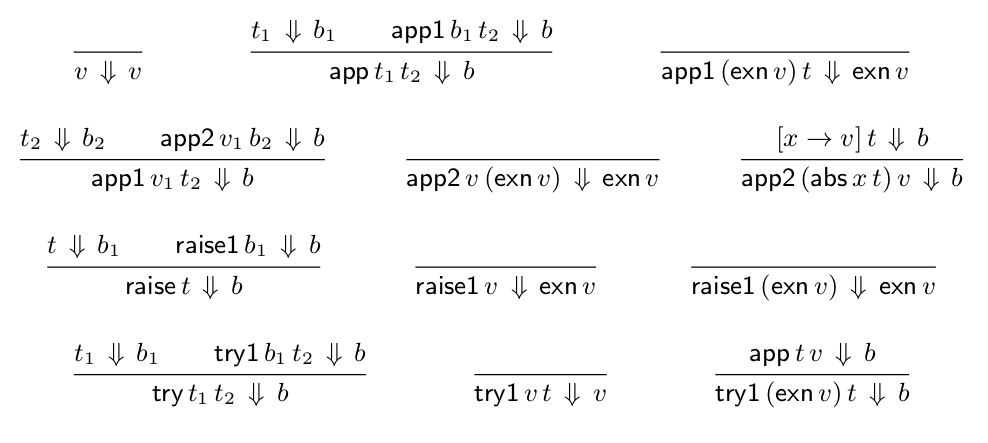
\includegraphics[scale=0.3]{ex_rules.png}
  \end{exampleblock}
\end{frame}

\begin{frame}{Divergence}
  outcome
\end{frame}

\begin{frame}{Coinduction}
  TODO: Chlipala examples
\end{frame}

\begin{frame}{Errors}
\end{frame}

\begin{frame}{Typing}
\end{frame}

\begin{frame}{Typing Soundness}
\end{frame}

\end{document}
